% Created 2020-03-07 Sat 11:51
% Intended LaTeX compiler: pdflatex
\documentclass[xcolor=table,10pt,aspectratio=169]{beamer}
\RequirePackage{etex}
\RequirePackage[l2tabu,orthodox]{nag}            %% Warn about obsolete commands and packages
\RequirePackage{amsmath,amsfonts,amssymb,amsthm} %% Math
\RequirePackage{ifxetex,ifluatex}                %% Detect XeTeX and LuaTeX
\RequirePackage{fixltx2e}                        %% provides \textsubscript
\RequirePackage{xspace}
\RequirePackage{graphicx}
\RequirePackage{comment}
\RequirePackage{url}
\RequirePackage{relsize}
\RequirePackage{booktabs}
\RequirePackage{tabularx}
\RequirePackage[normalem]{ulem}
\RequirePackage[all]{xy}
\RequirePackage{etoolbox}

%%%
%%% Code Listings
%%%

\RequirePackage{listings}
\lstdefinelanguage{Sage}[]{Python}{morekeywords={True,False,sage,cdef,cpdef,ctypedef,self},sensitive=true}

\lstset{frame=none,
  showtabs=False,
  showspaces=False,
  showstringspaces=False,
  commentstyle={\color{gray}},
  keywordstyle={\color{mLightBrown}\textbf},
  stringstyle ={\color{mDarkBrown}},
  frame=single,
  basicstyle=\tt\scriptsize\relax,
  backgroundcolor=\color{gray!190!black},
  inputencoding=utf8,
  literate={…}{{\ldots}}1,
  belowskip=0.0em,
}

\makeatletter
\patchcmd{\@verbatim}
  {\verbatim@font}
  {\verbatim@font\scriptsize}
  {}{}
\makeatother

%%%
%%% Tikz
%%%

\RequirePackage{tikz,pgfplots}

\usetikzlibrary{calc}
\usetikzlibrary{arrows}
\usetikzlibrary{automata}
\usetikzlibrary{positioning}
\usetikzlibrary{decorations.pathmorphing}
\usetikzlibrary{backgrounds}
\usetikzlibrary{fit,}
\usetikzlibrary{shapes.symbols}
\usetikzlibrary{chains}
\usetikzlibrary{shapes.geometric}
\usetikzlibrary{shapes.arrows}
\usetikzlibrary{graphs}

%% Cache

\ifdefined\tikzcaching  % chktex 1
  \usetikzlibrary{external}
  \tikzexternalize[prefix=build/]
  \tikzset{external/up to date check=diff}  %% MD5 fails from within emacs
\fi

%%%
%%% SVG (Inkscape)
%%%

\ifxetex % chktex 1
\newcommand{\executeiffilenewer}[3]{%
  {\immediate\write18{#3}} % hack
}
\else
\newcommand{\executeiffilenewer}[3]{%
  \ifnum\pdfstrcmp{\pdffilemoddate{#1}}%
    {\pdffilemoddate{#2}}>0%
    {\immediate\write18{#3}}
  \fi%
}
\fi

\newcommand{\includesvg}[2][1.0\textwidth]{%
 \executeiffilenewer{#1.svg}{#1.pdf}%
 {inkscape -z -D --file=#2.svg --export-pdf=#2.pdf --export-latex --export-area-page}%
 \def\svgwidth{#1} 
 \input{#2.pdf_tex}%
} 

%%%
%%% Metropolis Theme
%%%

\usetheme{metropolis}
\metroset{color/block=fill}
\metroset{numbering=none}
\metroset{outer/progressbar=foot}
\metroset{titleformat=smallcaps}

\setbeamercolor{description item}{fg=mLightBrown}
% \setbeamerfont{alerted text}{series=\bfseries}
\setbeamerfont{footnote}{size=\scriptsize}
\setbeamercolor{example text}{fg=mDarkBrown}
\setbeamercolor{block title alerted}{fg=white, bg=mDarkBrown}
\setbeamertemplate{bibliography item}[text]

\renewcommand*{\UrlFont}{\ttfamily\relax}

%%%
%%% UTF-8 & Fonts
%%% 

\RequirePackage{unicodesymbols} % after metropolis which loads fontspec

\setmonofont[BoldFont={Cousine Bold},
             ItalicFont={Cousine Italic},
             BoldItalicFont={Cousine Bold Italic},
             Scale=0.9]{Cousine}             
%%%
%%% BibLaTeX
%%%

\RequirePackage[backend=bibtex,
            style=alphabetic,
            maxnames=4,
            citestyle=alphabetic]{biblatex}

\bibliography{local.bib,abbrev3.bib,crypto_crossref.bib,rfc.bib,jacm.bib}

\DeclareFieldFormat{title}{\alert{#1}}
\DeclareFieldFormat[book]{title}{\alert{#1}}
\DeclareFieldFormat[thesis]{title}{\alert{#1}}
\DeclareFieldFormat[inproceedings]{title}{\alert{#1}}
\DeclareFieldFormat[incollection]{title}{\alert{#1}}
\DeclareFieldFormat[article]{title}{\alert{#1}}
\DeclareFieldFormat[misc]{title}{\alert{#1}}

%%% 
%%% Microtype
%%%

\IfFileExists{upquote.sty}{\RequirePackage{upquote}}{}
\IfFileExists{microtype.sty}{\RequirePackage{microtype}}{}

\setlength{\parindent}{0pt}                   %%
\setlength{\parskip}{6pt plus 2pt minus 1pt}  %%
\setlength{\emergencystretch}{3em}            %% prevent overfull lines
\setcounter{secnumdepth}{0}                   %%

%%% Local Variables:
%%% mode: latex
%%% End:
\usepackage{graphicx}
\usepackage{grffile}
\usepackage{longtable}
\usepackage{wrapfig}
\usepackage{rotating}
\usepackage[normalem]{ulem}
\usepackage{amsmath}
\usepackage{textcomp}
\usepackage{amssymb}
\usepackage{capt-of}
\usepackage{hyperref}
\usepackage{microtype}
\usepackage{newunicodechar}
\usepackage[notions,operators,sets,keys,ff,adversary,primitives,complexity,asymptotics,lambda,landau,advantage]{cryptocode}
\usepackage{xspace}
\usepackage{units}
\usepackage{nicefrac}
\usepackage{gensymb}
\usepackage{amsthm}
\usepackage{amsmath}
\usepackage{amssymb}
\usepackage{xcolor}
\usepackage{listings}
\usepackage[color=yellow!40]{todonotes}
\usetheme{default}
\author{Martin R. Albrecht}
\date{joint work with Alex Davidson, Amit Deo and Nigel Smart.}
\title{Round-optimal Verifiable Oblivious Pseudorandom Functions from Ideal Lattices}
\hypersetup{
pdfauthor={Martin R. Albrecht},
pdftitle={Round-optimal Verifiable Oblivious Pseudorandom Functions from Ideal Lattices},
pdfkeywords={},
pdfsubject={},
pdfcreator={Emacs 26.3 (Org mode 9.3.6)},
pdflang={English},
colorlinks,
citecolor=gray,
filecolor=gray,
linkcolor=gray,
urlcolor=gray
}
\begin{document}

\maketitle
\begin{frame}{Outline}
\tableofcontents
\end{frame}


\section{Motivation}
\label{sec:orgc236300}

\begin{frame}[label={sec:org776170f}]{VOPRF}
\procedure{}{%
\textbf{Client} \< \<  \textbf{Functionality} \< \< \textbf{Server}\\
\< \sendmessageright{top=\(m\)} \< \< \sendmessageleft{top=\(k\)} \<\\
\< \< \text{\(c = F_k(m)\)} \< \<\\
\< \sendmessageleft{top=\(c\)} \< \< \sendmessageright{top=\(\bot\)} \<\\
}
\end{frame}

\begin{frame}[label={sec:org9dae013}]{Applications: Privacy Pass I}
\begin{center}
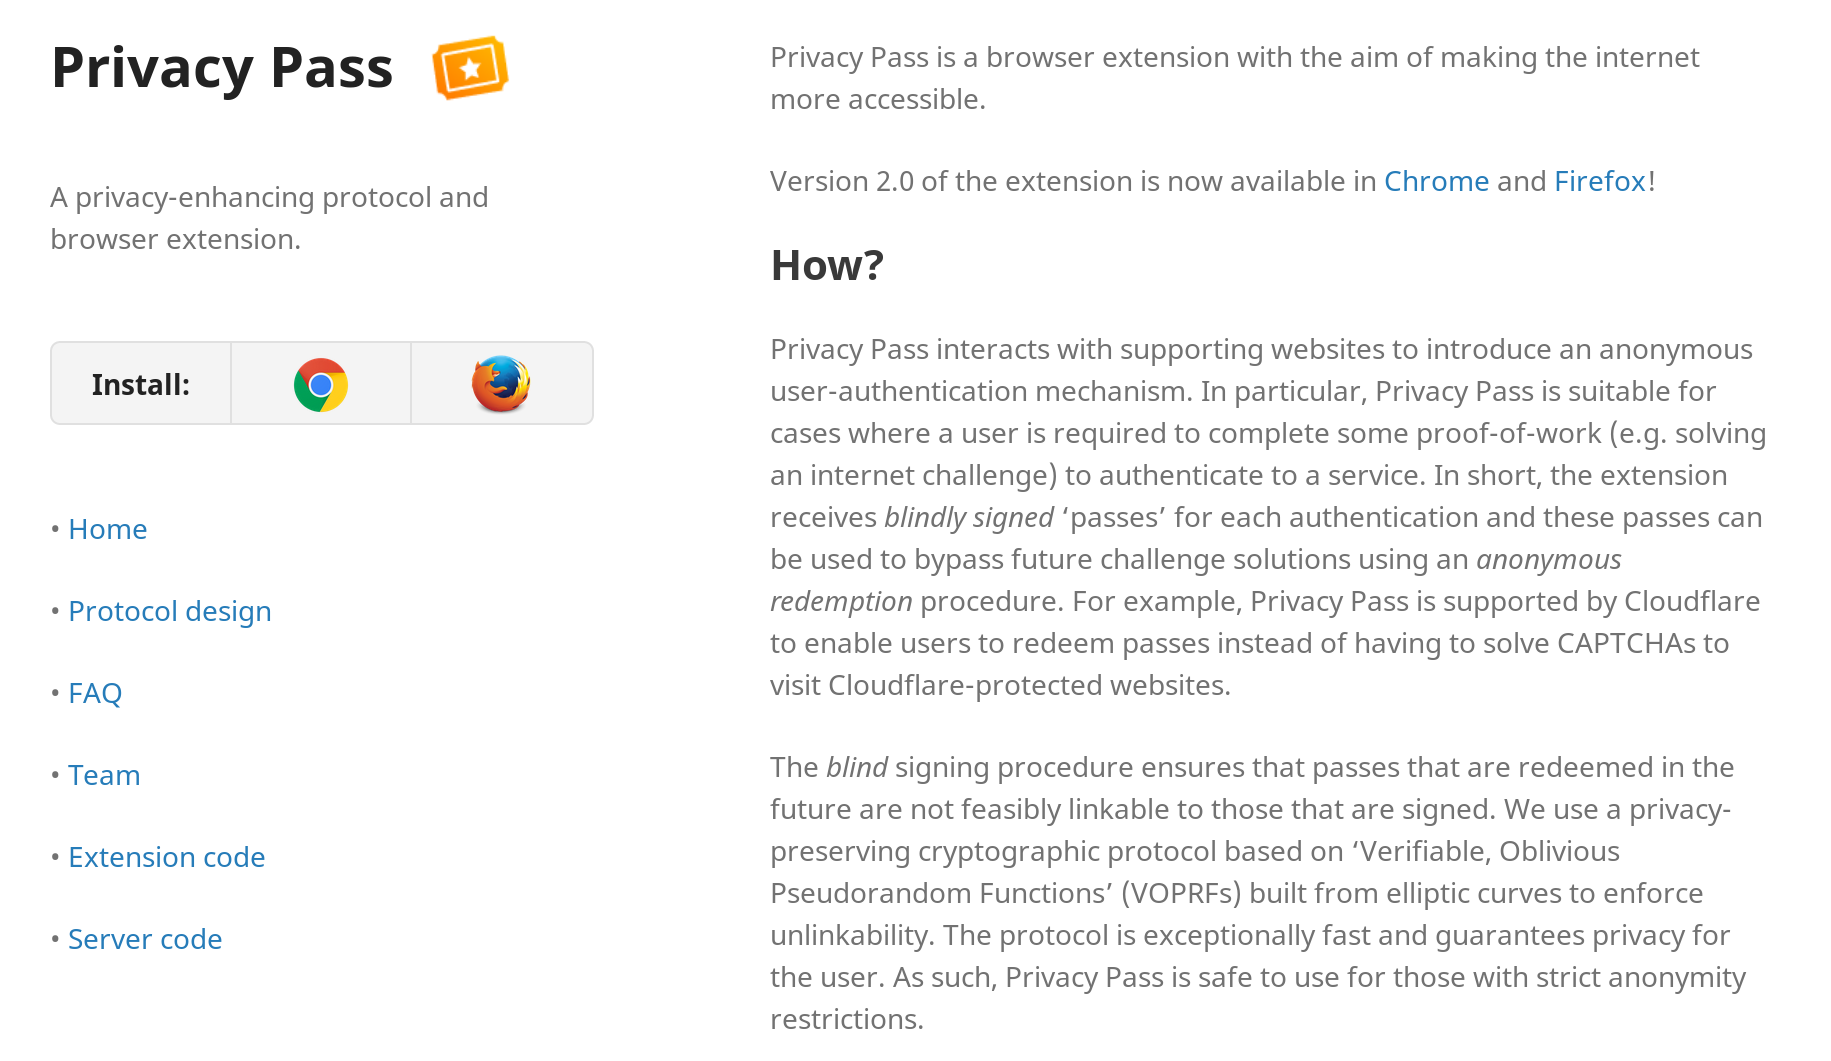
\includegraphics[width=0.8\linewidth]{./privacy-pass.png}
\end{center}
\end{frame}

\begin{frame}[label={sec:orga86bd12}]{Applications: Privacy Pass II}
\begin{columns}[t]
\begin{column}{0.6\columnwidth}
\textbf{Problem:}

\begin{itemize}
\item Tor users are having a hard time on Cloudflare protected sites
\item They’re constantly asked to solve CAPTCHAs to prove that they’re not bots
\item Want a privacy-preserving way of running reverse Turing test once and re-use later
\end{itemize}
\end{column}

\begin{column}{0.4\columnwidth}
\textbf{Idea:}

\begin{itemize}
\item Solve CAPTCHA
\item Evaluate a VOPRF on a bunch of random points to produce tokens \(F_k(x_i)\)
\item Redeem token by sending \((x_i, F_k(x_i))\)
\end{itemize}
\end{column}
\end{columns}

\vspace{1em}

\footnotesize
\fullcite{PoPETS:DGSTV18}
\end{frame}

\begin{frame}[label={sec:org4c89acc}]{Applications: OPAQUE}
\begin{columns}[t]
\begin{column}{0.5\columnwidth}
\textbf{Problem:}

\begin{itemize}
\item Passwords are everywhere,
\item but servers know passwords, e.g.
\begin{itemize}
\item phishing exploits that password are sent to server in clear
\item server breach
\item …
\end{itemize}
\end{itemize}
\end{column}

\begin{column}{0.5\columnwidth}
\textbf{Idea:}

\begin{description}
\item[{Registration}] Client stores \(Env_C = Enc_{rwd}(sk_C, pk_S)\) on server with \(rwd = F_k(pwd)\)
\item[{Login}] run OPRF \(rwd = F_k(pwd)\), client decrypts \(Env_C\) and runs key-exchange with \(S\).
\end{description}
\end{column}
\end{columns}

\vspace{1em}

\footnotesize
\fullcite{EC:JarKraXu18}
\end{frame}

\begin{frame}[label={sec:org6d7fb96}]{Applications: Other}
\begin{itemize}
\item Secure keyword search \footfullcite{TCC:FIPR05}
\item Private set intersection \footfullcite{TCC:JarLiu09}
\item Secure data de-duplication \footfullcite{USENIX:BelKeeRis13}
\item Password-protected secret sharing \footfullcite{ESP:JKKX16}
\end{itemize}
\end{frame}

\begin{frame}[label={sec:orgf5222ad}]{DH-Based VOPRF}
\centering
\procedure{}{%
\textbf{Client} \< \< \textbf{Server}\\
\< \sendmessageright*{\text{\(a = H(x) \cdot g^{r}\)}} \<\\
\< \sendmessageleft*{\text{\(b=a^k, v=g^k\)}} \<\\
\text{\(H(x)^k = b/v^r\)} \< \<\\
}

\[b/v^r = a^k/v^r = (H(x) \cdot g^{r})^k/(g^k)^r = H(x)^k\]
\end{frame}

\begin{frame}[label={sec:org861cc79}]{Standardisation}
\begin{columns}[t]
\begin{column}{0.6\columnwidth}
\begin{center}
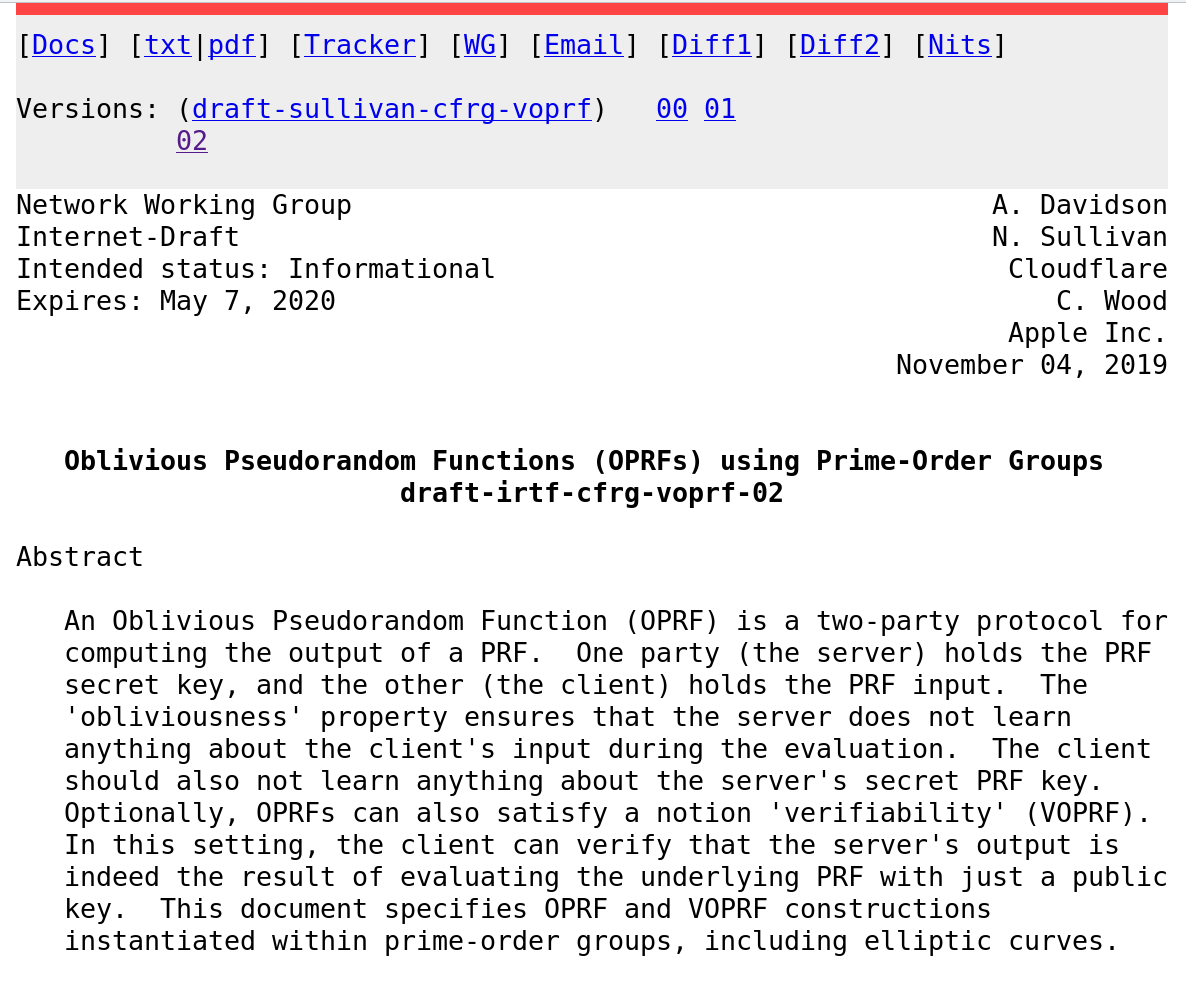
\includegraphics[width=\linewidth]{./draft-sullivan-cfrg-vopr.png}
\end{center}
\end{column}

\begin{column}{0.4\columnwidth}
\begin{itemize}
\item OPAQUE is currently being considered for standardisation
\item \alert<2>{DH-based} VOPRFs are currently being considered for standardisation
\end{itemize}
\end{column}
\end{columns}
\end{frame}

\begin{frame}[label={sec:orgc898ee1}]{VOPRFs in a Post-Quantum World}
\begin{center}
  \begin{tikzpicture}
    \node[anchor=south west,inner sep=0] (image) at (0,0) {
\includegraphics[width=0.9\textwidth]{shor.png}};
    \only<2>{\node[align=center,font={\Huge\bfseries},fill=white] at (image.center) {\alert{Bagga!}};}
  \end{tikzpicture}
\end{center}
\end{frame}

\section{A VOPRF from Lattices}
\label{sec:org09684cf}

\begin{frame}[label={sec:org59a6efc}]{Ring-LWE/Polynomial-LWE}
\begin{definition}
  Let \(q,n,\sigma> 0\) depend on \(\secpar\) (\(q,n\) are integers). The \textbf{decision-RLWE problem}\footfullcite{AC:SSTX09,EC:LyuPeiReg10} is to distinguish between:
  \[
  {(a_i,\ a_i \cdot s +e_i)} \in {(R_q)}^2\quad \text{ and }\quad  {(a_i,u_i)} \in {(R_q)}^2
  \]
  for \(a_i,u_i \sample R_q\); \(s,e_i \sample R(\chi_\sigma)\)
\end{definition}

\begin{itemize}
\item Think \(R_q = \ZZ_q[x]/(x^n+1)\) where \(n\) is a power of two.
\item \(\sample R(\chi_\sigma)\) returns elements with small coefficients.
\end{itemize}
\end{frame}

\begin{frame}[label={sec:orgd232589}]{1D-SIS}
\begin{definition} Let $ q,m,t $ depend on $ \secpar $. The
  \textbf{one-dimensional SIS problem}~\footfullcite{TCC:BraVai15} is: Given a uniform \( \mathbf{v} \sample \ZZ_q^m\), find \(\mathbf{z} \in \ZZ^m\) such that \( \|\mathbf{z}\|_\infty \leq t \) and \( \langle \mathbf{v}, \mathbf{z} \rangle \in [-t,t] + q \ZZ\).
\end{definition}

\begin{itemize}
\item Informally, the problem asks for a short element producing a short element when multiplied with a random vector.
\item The problem can be instantiated with vectors over the ring \(R_q\).
\end{itemize}
\end{frame}

\begin{frame}[label={sec:orge09296e}]{“Over Ideal Lattices”}
We have: If
\begin{description}
\item[{Ring-LWE}] is easy then finding short vectors in ideal lattices is easy on a quantum computer and if
\item[{1D-SIS}] is easy over rings then finding short vectors in ideal lattices is easy.
\end{description}

\pause

\begin{block}{Ideal-SVP}
At this point, we might have more confidence in Ring-LWE/Ring-SIS being hard on a quantum computer than Ideal-SVP.\footfullcite{EC:CraDucWes17}
\end{block}
\end{frame}

\begin{frame}[label={sec:orgb5b133b}]{VOPRF Blueprint}
\centering
\procedure{}{%
\textbf{Client} \< \< \textbf{Server}\\
\< \sendmessageright*{\text{\(a = H(x) \cdot g^{r}\)}} \<\\
\< \sendmessageleft*{\text{\(b=a^k, v=g^k\)}} \<\\
\text{\(H(x)^k = b/v^r\)} \< \<\\
}
\end{frame}

\begin{frame}[label={sec:org923d8f8}]{VOPRF Blueprint}
\centering
\procedure{}{%
\textbf{Client} \< \< \textbf{Server}\\
\< \sendmessageright*{\text{``\(F_r(x)\)''}} \<\\
\< \sendmessageleft*{\text{``\(g^a\)''}} \<\\
\text{\text{``\(g^{(a-b)}\)''}} \< \<\\
}
\end{frame}

\begin{frame}[label={sec:org8347acc}]{DH to Ring-LWE Dictionary}
\begin{center}
\begin{tabular}{ll}
DH Land & Ring-LWE Land\\
\hline
\(g\) & \(a\)\\
\(g^x\) & \(a\cdot s + e\)\\
 & \\
\(g^x \cdot g^y = g^{x+y}\) & \((a\cdot s + e_0) + (a \cdot t + e_1) = a \cdot (s+t) + e'\)\\
 & \\
\((g^a)^b = (g^b)^a\) & \((a\cdot s + e)\cdot t = (a\cdot s \cdot t + e \cdot t)\)\\
 & \(\approx a\cdot s \cdot t \approx (a\cdot t + e)\cdot s\)\\
 & assuming \(s\) and \(t\) are small\\
 & \\
\((g, g^a, g^b, g^{ab})\) & \((a,\ a\cdot s + e,\ a\cdot t + d,\ a \cdot s \cdot t + e')\)\\
\(\approx_c (g, g^a, g^b, u)\) & \(\approx_c (a,\ a\cdot s + e,\ a\cdot t + d,\ u)\)\\
\end{tabular}

\end{center}
\end{frame}

\begin{frame}[label={sec:org332728c}]{(Ring-)LWR: Derandomised (Ring-)LWE}
Ring-LWE effectively overwrites the lower order bits of \(a\cdot s\) with \(e\). Ring-LWR simply drops those bits.

\begin{definition}
  Let \(q,n,p\) depend on \(\secpar\) be integers and \(p \mid q\). The \textbf{decision-RLWR problem} is to distinguish between:
  \[
  {\left(a_i,\ \left\lfloor \frac{p}{q} \cdot a_i \cdot s \right\rceil\right)} \in {(R_q,R_p)} \quad \text{ and }\quad  {(a_i,u_i)} \in {(R_q,R_p)}
  \]
  for \(a_i \sample R_q\), \(s \sample R(\chi_\sigma)\), \(u_i \sample R_p\).
\end{definition}

The security of LWR can be reduced to LWE.
\end{frame}

\begin{frame}[label={sec:org6fcdebc}]{LWR-Based PRF: BP14 I}
For a particular function \(\mathbf{a}^F: {\{0,1\}}^L \rightarrow R_q^{1\times \ell}\) we set out to design a VOPRF for the PRF 
\[
F_k(x) = \left\lfloor \frac{p}{q} \cdot \mathbf{a}^F(x) \cdot k \right\rceil
\] 
where the key \(k \in R_q\) is small.

\begin{block}{}
\fullcite{C:BanPei14}
\end{block}
\end{frame}

\begin{frame}[label={sec:orgc9b1a06}]{LWR-Based PRF: BP14 II}
\begin{columns}[t]
\begin{column}{0.5\columnwidth}
As an example, consider the PRF for 2-bit inputs.

We define \(\mathbf{a}^F(x) = \mathbf{a}_{x_0} \cdot G^{-1}\left( \mathbf{a}_{x_1}\right)\)  where 

\begin{itemize}
\item \(\mathbf{a}_0, \mathbf{a}_1 \in R_q^{1\times \ell}\) are uniform,
\item \(G^{-1}\left( \mathbf{a}_2 \right) \in R_2^{\ell \times \ell}\) is binary decomposition,
\item \(G = (1,2,\dots, 2^{\ell-1})\).
\end{itemize}
\end{column}

\begin{column}{0.5\columnwidth}
\textbf{Example}:

\begin{itemize}
\item \(x = 5 \bmod 8\)
\item \(G^{-1}(5) = (1, 0, 1)\)
\item \(G \cdot (1, 0, 1) = (1, 2, 4) \cdot (1, 0, 1) = 1 + 4 = 5\)
\end{itemize}
\end{column}
\end{columns}
\end{frame}

\begin{frame}[label={sec:org8b297b0}]{LWR-Based PRF: BP14 III}
We can write 
\begin{align*}
\left\lfloor \frac{p}{q} \cdot \mathbf{a}^F(x) \cdot k \right\rceil &= \left\lfloor \frac{p}{q} \cdot k\cdot \mathbf{a}_{x_0} \cdot G^{-1}(\mathbf{a}_{x_1}) \right\rceil 
= \left\lfloor \frac{p}{q} \cdot (k\cdot \mathbf{a}_{x_0} + \mathbf{e})\cdot G^{-1}(\mathbf{a}_{x_1}) \right\rceil \\
&\approx_c \left\lfloor \frac{p}{q}\cdot\mathbf{u}\cdot G^{-1}(\mathbf{a}_{x_1}) \right\rceil \text{ (RLWE)}\\
&= \left\lfloor \frac{p}{q} (u'G+\mathbf{e}') \cdot G^{-1}(\mathbf{a}_{x_1}) \right\rceil = \left\lfloor \frac{p}{q} \left(u' \mathbf{a}_{x_1} + \mathbf{e}''\right) + \frac{p}{q} \mathbf{e}' \cdot G^{-1}(\mathbf{a}_{x_1}) \right\rceil \\ 
&\approx_c \left\lfloor \frac{p}{q} \cdot \mathbf{u}'' + \frac{p}{q} \cdot \mathbf{e}' \cdot G^{-1}(\mathbf{a}_{x_1}) \right\rceil \text{ (RLWE)} \\
& = \left\lfloor \frac{p}{q} \cdot \tilde{\mathbf{u}} \right\rceil
\end{align*}
where \(\mathbf{u}, \mathbf{u}'',  \tilde{\mathbf{u}}\) are uniform in \(R_q^{1 \times \ell}\), \(u'\) is uniform in \(R_q\) and  uniform \(\mathbf{e}' \in R_q^{1 \times \ell} / (R_q \cdot G)\).
\end{frame}

\begin{frame}[label={sec:orgcb935fe}]{A First Attempt}
\begin{center}
\procedure{}{%
\textbf{Client} \< \< \textbf{Server}\\
\< \sendmessageright*{\text{\(\mathbf{c}_x = \mathbf{a}^F(x) \cdot r + \mathbf{e}\)}} \<\\
\< \sendmessageleft*{\text{\(\mathbf{d}_x = \mathbf{c}_x \cdot k + \mathbf{e}'\)}} \<\\
\text{\(\left\lfloor \frac{p}{q} \cdot \mathbf{d}_x \cdot r^{-1} \right\rceil \)} \< \<\\
}
\end{center}

We \textbf{would like to say} that \[\left\lfloor \frac{p}{q} \cdot \mathbf{d}_x \cdot r^{-1} \right\rceil = \left\lfloor  \frac{p}{q}\cdot \mathbf{a}^F(x) \cdot k + \frac{p}{q}\left(\mathbf{e}\cdot k\cdot r^{-1} + \mathbf{e}'\cdot  r^{-1}\right) \right\rceil = \left\lfloor \frac{p}{q} \cdot \mathbf{a}^F(x)\cdot k \right\rceil. \]
\end{frame}

\begin{frame}[label={sec:org97073f8}]{Problem 1}
\begin{columns}[t]
\begin{column}{0.5\columnwidth}
\begin{itemize}
\item This simplified protocol cannot be realised using standard RLWE secret distributions.
\item The problem is that there is no standard RLWE secret distribution where samples from the distribution are guaranteed to have \alert{small inverses} in \(R_q\).
\end{itemize}
\end{column}

\begin{column}{0.5\columnwidth}
\textbf{Secret distribution}:

\begin{description}
\item[{uniform}] fine
\item[{error distribution}] fine
\item[{small}] fine, small loss
\item[{\(s^{-1}\) small}] maybe fine, but not proven
\end{description}
\end{column}
\end{columns}
\end{frame}


\begin{frame}[label={sec:org697e68a}]{“Every problem in computer science can be solved by adding another layer of indirection”}
\begin{enumerate}
\item Sample small ring elements \(s\) and \(t\).
\item Run the extended GCD algorithm to compute \alert{some} \(u'\cdot s + v'\cdot t = 1\).
\item Observe that \[(u' - r \cdot t)\cdot s + (v'+ r \cdot s)\cdot t = u'\cdot s - r \cdot t \cdot s + v'\cdot t + r \cdot s\cdot t = 1\]
\item Use Babai’s rounding algorithm to find \(r\) s.t. \(u = u' - r \cdot s\) and \(v = v' + r\) are small.
\end{enumerate}

\begin{block}{Result}
\begin{center}
We end up with \(u \cdot s + v \cdot t = 1 \bmod R_q\) where \(u,s,v,t\) are all small.\footfullcite{RSA:HHPSW03,EPRINT:PorPre19}
\end{center}
\end{block}
\end{frame}

\begin{frame}[label={sec:orgad0c1f8}]{A Second Attempt}
\begin{center}
\procedure{}{%
\textbf{Client} \< \< \textbf{Server}\\
\< \sendmessageright*{\text{\(\mathbf{c}_x^1 = \mathbf{a}^F(x) \cdot s + \mathbf{e}_1, \quad \mathbf{c}_x^2 = \mathbf{a}^F(x) \cdot t + \mathbf{e}_2\)}} \<\\
\< \sendmessageleft*{\text{\(\mathbf{d}_x^1 = \mathbf{c}_x^1 \cdot k + \mathbf{e}'_1, \quad \mathbf{d}_x^2 = \mathbf{c}_x^2 \cdot k + \mathbf{e}'_2\)}} \<\\
\text{\(\left\lfloor \frac{p}{q} \cdot  \left(u \cdot \mathbf{d}_x^1 + v \cdot \mathbf{d}_x^2 \right) \right\rceil \)} \< \<\\
}
\end{center}

We \textbf{can} that \[\left\lfloor \frac{p}{q} \cdot  \left(u \cdot \mathbf{d}_x^1 + v \cdot \mathbf{d}_x^2 \right) \right\rceil = 
\left\lfloor \frac{p}{q} \cdot  \left(u \cdot \mathbf{a}^F(x) \cdot s \cdot k + v \cdot \mathbf{a}^F(x) \cdot t \cdot k \right) + \frac{p}{q} \mathbf{e}' \right\rceil = \left\lfloor \frac{p}{q} \cdot \mathbf{a}^F(x) \cdot k \right\rceil\]
\end{frame}

\begin{frame}[label={sec:org579df9b}]{Problem 2}
\begin{definition}
  Let \(q,n,\sigma > 0\) depend on \(\secpar\) (\(q,n\) are integers). The \textbf{NTRU problem} is to distinguish between:
  \[f/g \in R_q \quad \text{ and }\quad u \in R_q\]
  for \(f,g \sample R(\chi_\sigma)\), \(g\) invertible in \(R_q\) and \(u \sample R_q\).
\end{definition}

\textbf{Attack:}

\begin{itemize}
\item Client sends \(c_x^1 = \gamma\cdot f/g\) for some scalar \(\gamma\).
\item Server sends \(d_x^1  = c_x^1 \cdot k + e'_1\)
\item Client computes \(d_x^1\cdot g = (\gamma\cdot f/g \cdot k + e'_1) \cdot g = \gamma\cdot f\cdot k +  e'_1 \cdot g\)
\end{itemize}
\end{frame}

\begin{frame}[label={sec:orgdbe1364}]{Our Construction}
\begin{center}
\procedure{}{%
\textbf{Client} \< \< \textbf{Server}\\
\< \sendmessageright*{\text{\(\mathbf{c}_x^1 = \mathbf{a}^F(x) \cdot s + \mathbf{e}_1, \quad \mathbf{c}_x^2 = \mathbf{a}^F(x) \cdot t + \mathbf{e}_2\)}} \<\\
\< \sendmessageright*{\text{``proof'' \(\pi_{1}\) that \(\mathbf{c}_x^1, \mathbf{c}_x^2\) are well-formed.}} \<\\
\< \< \text{Check \(\pi_{1}\)}\\
\< \sendmessageleft*{\text{\(\mathbf{d}_x^1 = \mathbf{c}_x^1 \cdot k + \mathbf{e}'_1, \quad \mathbf{d}_x^2 = \mathbf{c}_x^1 \cdot k + \mathbf{e}'_2\)}} \<\\
\< \sendmessageleft*{\text{``proof'' \(\pi_{2}\) that \(\mathbf{d}_x^1, \mathbf{d}_x^2\) are well-formed.}} \<\\
\text{Check \(\pi_{2}\)} \< \<\\
\text{\(\left\lfloor \frac{p}{q} \cdot  \left(u \cdot \mathbf{d}_x^1 + v \cdot \mathbf{d}_x^2 \right) \right\rceil \)} \< \<\\
}
\end{center}
\end{frame}

\section{Security}
\label{sec:org064770c}

\begin{frame}[label={sec:orgd531389}]{Notion}
A protocol \(\Pi\) is a verifiable oblivious pseudorandom function if all of the following hold:

\begin{description}
\item[{Correctness}] the protocol outputs the correct evaluation with overwhelming probability
\item[{Malicious server}] a malicious server cannot tell if it s talking to the ideal functionality or \(\Pi\)
\item[{Average case malicious client}] \textbf{for a random \(k\)} a malicious client cannot tell if it is talking to the ideal functionality or \(\Pi\)
\end{description}
\end{frame}

\begin{frame}[label={sec:org767252a}]{Client Security: RLWE \& 1D-SIS}
\begin{itemize}
\item The messages \(\mathbf{c}_x^1 = \mathbf{a}^F(x) \cdot s + \mathbf{e}_1\) and  \(\mathbf{c}_x^2 = \mathbf{a}^F(x) \cdot t + \mathbf{e}_2\) are indistinguishable from uniform by RLWE assumption.
\item Correctness holds by the 1D-SIS assumption.
\end{itemize}
\end{frame}

\begin{frame}[label={sec:orgffd75af}]{Server Security: RLWE \& Drowning}
\begin{itemize}
\item Note that \[\mathbf{d}_x^1 = \mathbf{a}^F(x) \cdot s \cdot  k + \mathbf{e}_1 \cdot k + \mathbf{e}_1'\]
\item If we pick \(\mathbf{e}'_1\) from a distribution that hides addition of terms \(\mathbf{e} \cdot k\) and \(\mathbf{e}_s \cdot s\) (where \(\mathbf{e}_s\) is identically distributed to \(\mathbf{e}\)) then
\item from the perspective of the client, the server might as well have sent \[\mathbf{d}_x^1 = (\mathbf{a}^F(x) \cdot k + \mathbf{e}_s) \cdot s + \mathbf{e}_1'.\]
\item The term in brackets \(\mathbf{a}^F(x) \cdot k + \mathbf{e}_s\) computationally indistinguishable from uniform random under a RLWE assumption
\item Thus, the message \(\mathbf{d}_x^1\) leaks nothing about the server's key \(k\).
\end{itemize}
\end{frame}

\section{Parameters}
\label{sec:org4f51708}

\begin{frame}[label={sec:org771ccc5}]{They’re Disgusting!}
\begin{itemize}
\item We need super-polynomial \(q\) for BP14 and we need super-polynomial \(q\) for drowning
\begin{itemize}
\item \(\secpar = 128 \Rightarrow q = 2^{256}\)
\end{itemize}
\item Need  \footfullcite{JMC:AlbPlaSco15} LWE dimension \(n = 2^{14}\)
\begin{itemize}
\item \(2^{22}\) bits per RLWE sample: 0.5MB, need two samples per direction
\end{itemize}
\end{itemize}

\begin{block}{ZK Cost}
This is ignoring the cost of sending the zero-knowledge arguments
\end{block}

But can tune parameters, round more aggressively, perhaps remove drowning …
\end{frame}

\section{Alternative Constructions}
\label{sec:org0493321}

\begin{frame}[label={sec:orgdf1767e}]{Alternative VOPRF Candidate: Prove a Hash Function}
\begin{itemize}
\item Let \(H(\cdot)\) be a zk-friendly hash function \footfullcite{EC:ARSTZ15,AC:AGRRT16,EPRINT:AABDS19}
\item Prove \(\mathsf{seed} = H(x)\) instead of proving \(\mathbf{a}^F(x) \cdot s + e\).
\item Let \(\mathbf{a}_{\mathsf{seed}}\) is the output of some sampler \footfullcite{USENIX:ADPS16} of elements in \(R_q\) when given  \(\mathsf{seed}\) as input
\item Send \((\mathsf{seed}, \mathbf{a}_{\mathsf{seed}} \cdot s + e)\)
\item Still need to prove \(\mathbf{a}_{\mathsf{seed}} \cdot s + e\) but this is easier/cheaper.
\end{itemize}
\end{frame}

\begin{frame}[label={sec:org0156a7a}]{Alternative VOPRF Candidate: FHE}
\begin{enumerate}
\item Client encrypts \(x\) under an FHE scheme
\item Sever computes \(Eval(F_k, x)\) homomorphically using an FHE friendly PRF \footfullcite{EC:ARSTZ15,AC:AGRRT16,EPRINT:AABDS19}
\item Client decrypts \(F_k(x)\).
\end{enumerate}
\end{frame}

\begin{frame}[label={sec:org7b8b6ca}]{Alternative Applications aka “We will miss DH”}
\begin{itemize}
\item NIST PQ {\color{lightgray}{Competition} }Process only covers ephemeral key exchange and digital signature schemes
\item VOPRFs are just one example of DH-based constructions that need translation in a post-quantum world
\item We cannot even do an efficient post-quantum NIKE
\end{itemize}
\end{frame}

\begin{frame}[label={sec:org866bc91},standout]{Fin}
\begin{center}
\Huge \alert{Thank You}
\end{center}

PS: We are hiring a lecturer/assistant professor in the ISG. \url{https://jobs.royalholloway.ac.uk/0120-023} Application deadline: 15 April

PPS: We are looking for PhD students. \url{https://royalholloway.ac.uk/CDT}
\end{frame}
\end{document}